%%%%%%%%%%%%%%%%%%%%%%%%%%%%%%%%%
% Please read the IEEE standard 829-1998 document before starting and describing your experiments.
% The document is available SVN, file name IEEE829_1998.pdf
% The XtreemOS evaluation reports will mainly follow the structure and recommendation of IEEE.
%%%%%%%%%%%%%%%%%%%%%%%%%%%%%%%%%

% please add name of component tested
\section{Evaluation of XtreemOS API : SAGA}
 \label{sec:eval-api}


% Tests will be done with MODERATO or ZEPHYR.\\
 %Responsible for tests and documentation:  Samuel (EDF).

%{\huge {\bf Still under construction!!!!}}

 % please add name of component tested

%  \subsection{What is SAGA?}

%  {\bf Notice: } The presented information is taken from the SAGA
%  web site: \\
%  \begin{center}
%   \mbox{\href{https://mail.cct.lsu.edu/mailman/listinfo/saga-users
%  }{https://mail.cct.lsu.edu/mailman/listinfo/saga-users}} \end{center}
%  In the following paragraphs, every verbatim quotation of this site
%  is written in slanted text.
   

    SAGA stands for ``a Simple API for Grid Application''. It 
    is an application level programming abstraction that
    builds on the top of XtreemOS or of grid middleware such as Globus
    or OMII-UK. %\fix{[Bernd] XtreemOS is not Grid middleware}
  
   \begin{figure}[h]
    \begin{center}
     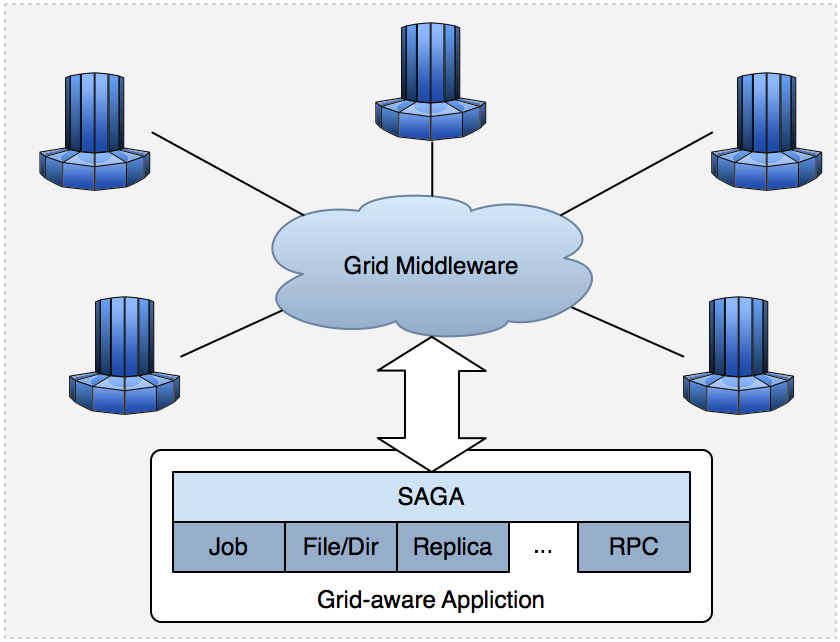
\includegraphics[width=8cm]{figures/saga.png}
    \end{center}   
   \end{figure}


%    \begin{sl}

%     The lack of such application-level programming abstractions is
%     compounded by the fact that there exist incompatible and often changing
%     Grid middleware systems in both research and production environments.
%     To address these challenges and in particular to find a solution to the
%     universal, apparently intractable problem of successfully Grid-enabling
%     applications, several applications groups expressed the desire for a
%     simple programmatic interface that is widely-adopted, usable and
%     available.  The goal of such an interface would be to provide a ``grid
%     counterpart to MPI'' (at least in impact if not in details) and that
%     would supply developers with a simple, uniform, and standard
%     programmatic interface with which to develop distributed applications.
%     Thanks to the efforts of many contributors, an initial specification of
%     such a ``grid counterpart to MPI'' now exists -- the Simple API for Grid
%     Applications (SAGA). SAGA is now on the threshold of becoming an Open
%     Grid Forum (OGF) technical recommendation (early 2008).
%     \\

%     SAGA has the following properties:
%     \begin{itemize}
%      \item Simplicity: easy to use, install, administer and maintain
%      \item Uniformity: provides support for different application programming languages as well as consistent semantics and style for different Grid functionality
%      \item Scalability: Contains mechanisms for the same application (source) code to run on a variety of systems ranging from laptops to HPC resourcesGenericity: adds support for different grid middleware, even concurrent ones
%      \item Modularity: provides a framework easily extendable
%     \end{itemize}
%    \end{sl}



    Two SAGA implementations  -- in C++ and Java --  have been planned as
    well as wrappings in C, fortran, Python and Perl. The only 
    technical requirement is the availability of the library boost
    in a version higher than 1.33.

    The 0.6 and 0.7 versions of the C++ implementation (``SAGA-A'') have been
    respectively released in June and November 2007. SAGA is the
    latest Open Source adoption of the GWD-R.90 (SAGA Core API) standard. It
    provides a Grid programming API for the six functional
    packages defined by GWD-R90 1.0:
    \begin{itemize}
     \item Replica Management
     \item Job Management
     \item Namespaces
     \item File Management
     \item Remote Procedure Call
     \item Streams
    \end{itemize}
%    Additionally, this implementation includes proof of concept implementations (including default adaptors) of proposed API extensions which will most likely become part of future releases / extensions of the standard:
%    \begin{itemize}
%     \item Advert Service 
%    \end{itemize}
    

    %here enter brief introduction: name of component, description, WP
    %responsible...

  \subsection{XtreemOS SAGA Implementation}

  In XtreemOS project, workpackage {\bfseries WP 3.1} is responsible
  for the porting of SAGA. The first release of an XtreemOS component is
  planned for February 2008. 


  Though the XtreemOS component is not yet available, one can already 
  have a fair idea of the completeness of the API 
  and the fulfillment of the requirements by reading the published
  specification of SAGA and by experimenting with it running only on a
  standard Linux Box. % \fix{[Bernd] what do you mean by ``default compiling''?}

  %first, one test plan
  \inputexpfile{wp31-api-ts01-tp.tex}
  %depending on the test plan, the following documents may be used multiple times, please arrange in meaningful order
  \inputexpfile{wp31-api-ts01-zephyr01-tds01.tex}
  \inputexpfile{wp31-api-ts01-zephyr01-tcs01.tex}
  \inputexpfile{wp31-api-ts01-zephyr01-tps01.tex}
  \inputexpfile{wp31-api-ts01-zephyr01-tl01.tex}
  \inputexpfile{wp31-api-ts01-zephyr01-tir01.tex} 
   \inputexpfile{wp31-api-ts01-zephyr01-tcs02.tex}
  \inputexpfile{wp31-api-ts01-zephyr01-tps02.tex}
  \inputexpfile{wp31-api-ts01-zephyr01-tl02.tex}

  %finally, one test summary report
  \inputexpfile{wp31-api-ts01-tsr.tex}

